\documentclass[11pt,a4paper,final]{article}
\usepackage[utf8]{inputenc}
\usepackage[T1]{fontenc}
\usepackage{amsmath}
\usepackage{amsfonts}
\usepackage{mathtools}
\usepackage{amssymb}
\usepackage{bm,bbm}
\usepackage[final]{graphicx}
\graphicspath{{./images/}}
\usepackage{caption}
\usepackage{subcaption}
\usepackage[usenames, dvipsnames]{color}
\usepackage[margin=1in]{geometry} % to adjust the page margins
%\pagenumbering{gobble} % To suppress page numbering 

\DeclarePairedDelimiterX{\norm}[1]{\lVert}{\rVert}{#1}
\newcommand{\seminorm}[1]{\left\lvert #1 \right\rvert}

\usepackage{breqn}
\usepackage{empheq}
\usepackage[most]{tcolorbox}

\usepackage{tikz,pgfplots}
\usetikzlibrary{spy}
\pgfplotsset{table/search path={./data}} %checks in data folder
\pgfplotsset{compat=newest}	%mention version to avoid warnings
\pgfplotsset{every axis/.append style={
                    label style={font=\small},
                    legend style={font=\small, draw=none, fill=none},
                    tick label style={font=\small}
                    }}

\usepackage{array}                            % better table support
\newcolumntype{C}[1]{>{\centering\arraybackslash}m{#1}}
\usepackage{multicol}                         % spanning columns
\usepackage{multirow}                         % spanning rows
\usepackage[ruled,vlined]{algorithm2e}
\usepackage{stmaryrd} % for jump in gradient symbol
\usepackage{siunitx}
\usepackage{textcomp} % for trademark and registered symbols
\usepackage[capitalise, noabbrev]{cleveref}
\usepackage[backend=biber,style=numeric,sorting=ynt]{biblatex}
\addbibresource{task2_ref.bib}

\begin{document}
\begin{center}
\textbf{\Large Master thesis: documentation of task 2.2}\\ \vspace{0.25cm}
\textbf{\large Vinayak Gholap}
\end{center}

\section{Tasks performed}
\begin{enumerate}
\item abc
\end{enumerate}

\section{Introduction}
Coupled magneto-elasticity problem. Multi-physics theory, arising difficulties, challenges in modelling. Summarising results and conclusions from task 1 and 2.1. 

\section{Constitutive material model for coupled problem}
The material response is characterised by a Helmholtz free energy density function. For the considered magneto-elastic material, in addition to the dependence on the deformation gradient $\mathbf{F}$ and the Jacobian $J$ (as already seen in quasi-static finite strain compressible elasticity, Task 2.1), the free energy density function now also depends on the referential magnetic vector field. The strain energy function (S.E.F.) is given as: 
\begin{equation}
\Psi = \Psi (J, \mathbf{F}, \mathbb{H}) = \Psi (J, \mathbf{C}, \mathbb{H}).
\label{eq:3.1}
\end{equation}
Using the symmetry argument from the definition of the right Cauchy-Green deformation tensor $\mathbf{C} := \mathbf{F}^T \cdot \mathbf{F}$, the dependence of $\mathbf{F}$ is simplified to a dependence on $\mathbf{C}$. The isotropic hyperelastic material response when $\mathbf{C}$ is used to describe the S.E.F. is given by the constitutive relation as
\begin{equation}
\mathbf{S} = 2 \dfrac{\partial \Psi (J, \mathbf{C}, \mathbb{H})}{\partial \mathbf{C}}.
\label{eq:3.2}
\end{equation}
The referential magnetic induction vector field $\mathbb{B}$ is modelled in terms of the referential magnetic vector field $\mathbb{H}$, taking $\mathbb{H}$ as the independent field
\begin{equation}
\mathbb{B} = \mathbb{B}(\mathbb{H}),
\label{eq:3.3}
\end{equation}
which is termed as the alternative formulation in \cite{dorfmann2004}. With $\mathbb{H}$ chosen as the independent field, its components can be chosen to satisfy the vector equation $\text{Curl} \mathbb{H} = \mathbf{0}$ and then the resulting $\mathbb{B}$ has to satisfy the scalar equation $\text{Div} \mathbb{B} = 0$. This alternative formulation does not put restrictions on the admissible class of constitutive laws (which arise if one were to proceed with $\mathbb{B}$ as the independent field) and also avoids the complexities of a vector-valued magnetic field from the finite element modelling aspects. The fundamental constitutive equation that relates the magnetic quantities $\mathbb{B}, \mathbb{H}$ and the magnetization vector $\mathbb{M}$ is given as \cite{dorfmann2004,dorfmann2005}
\begin{equation}
J^{-1} \mathbf{C} \cdot \mathbb{B} = \mu_0 \left[ \mathbb{H} + \mathbb{M} \right].
\label{eq:3.3.2}
\end{equation}
The magnetization vector field exists only in the solid magneto-elastic material and vanishes in the free space. $\mathbb{B}$ is given by another constitutive relation as \cite{dorfmann2004}: 
\begin{equation}
\mathbb{B} = -\dfrac{\partial \Psi (J, \mathbf{C}, \mathbb{H})}{\partial \mathbb{H}}.
\label{eq:3.4}
\end{equation}
The S.E.F corresponding to a compressible coupled magneto-elastic Neo-Hookean material is given as: 
\begin{align}
\Psi (J, \mathbf{C}, \mathbb{H}) &= \dfrac{\mu}{2} \left[ \mathbf{C} : \mathbf{I} - \mathbf{I} : \mathbf{I} -2 \ln J \right] + \dfrac{\lambda}{2} (\ln J)^2 \textcolor{red}{- \frac{\mu_0 \mu_r}{2} [J \mathbf{C}^{-1} : \mathbb{H} \otimes \mathbb{H}]}, \\
&= \Psi_0^{\text{elas}} (\mathbf{C}) + \mu_r M_0 (J, \mathbf{C}, \mathbb{H}), \\
& \text{with} \ M_0 (J, \mathbf{C}, \mathbb{H}) := -\frac{\mu_0}{2} [J \mathbf{C}^{-1} : \mathbb{H} \otimes \mathbb{H}],
\label{eq:3.5}
\end{align}
where $\mu$ and $\nu$ are the Lam\'e parameters, $\mu_0 = 4 \pi \times 10^{-7} \ \text{Hm}^{-1}$ is the free space (vacuum) magnetic permeability and $\mu_r$ is the relative magnetic permeability of the magneto-elastic material ($\mu_r = 1$ represents the free space material). The term highlighted in red takes into account the energy stored in the body due to applied external magnetic load $\mathbb{H}$ and the response of the coupled interaction between the displacement field and the magnetic field. The term $\Psi_0^{\text{elas}} (\mathbf{C})$ describes the purely elastic response of the material and the term $M_0 (J, \mathbf{C}, \mathbb{H})$ describes the total energy per unit volume stored in the magnetic fields in the free space \cite{dorfmann2004}. The constant $\mu_r > 1$ represents a magnetisable material such as the membrane. \par 

The second Piola-Kirchhoff stress $\mathbf{S}$ for the considered S.E.F. as stated in \Cref{eq:3.5} is derived below.
\begin{align*}
\mathbf{S} &= 2 \dfrac{\partial \Psi (J, \mathbf{C}, \mathbb{H})}{\partial \mathbf{C}} \\
&= 2 \left[ \dfrac{\mu}{2} \left\lbrace \dfrac{\partial [\mathbf{C} : \mathbf{I}]}{\partial \mathbf{C}} - 2 \dfrac{\partial \ln J}{\partial \mathbf{C}} \right\rbrace + \dfrac{\lambda}{2} \dfrac{\partial (\ln J)^2}{\partial \mathbf{C}} - \dfrac{\mu_0 \mu_r}{2} \dfrac{\partial [J \mathbf{C}^{-1} : \mathbb{H} \otimes \mathbb{H}]}{\partial \mathbf{C}} \right]
\end{align*}
Side calculation 1:
\begin{align*}
\dfrac{\partial [\mathbf{C} : \mathbf{I}]}{\partial \mathbf{C}} &= \mathbf{I} \\ 
\dfrac{\partial \ln J}{\partial \mathbf{C}} &= \dfrac{1}{J} \dfrac{\partial J}{\partial \mathbf{C}} \\
\dfrac{\partial (\ln J)^2}{\partial \mathbf{C}} &= 2 \ \ln J \ \dfrac{\partial \ln J}{\partial \mathbf{C}} \\
\dfrac{\partial J}{\partial \mathbf{C}} &= \dfrac{1}{2} J \mathbf{C}^{-1} \ \  \text{c.f. \cite[see][page 46 Equation (3.124)]{Wriggers2008}}
\end{align*}
\begin{align*}
\mathbf{S} &= \mu \mathbf{I} -  \mu \mathbf{C}^{-1} + \lambda \ln J \mathbf{C}^{-1} - \mu_0 \mu_r \dfrac{\partial [J \mathbf{C}^{-1} : \mathbb{H} \otimes \mathbb{H}]}{\partial \mathbf{C}}
\end{align*}
Side calculation 2: Note $\mathbf{C} := \mathbf{F}^T \cdot \mathbf{F} \ $ is symmetric $\implies \mathbf{C}^{-1}$ is also symmetric 
\begin{align*}
\dfrac{\partial [J \mathbf{C}^{-1} : \mathbb{H} \otimes \mathbb{H}]}{\partial \mathbf{C}} &= \dfrac{\partial [J C^{-1}_{IJ} H_I H_J]}{\partial C_{KL}} \ \mathbf{E}_K \otimes \mathbf{E}_L \\
&= C^{-1}_{IJ} \ H_I \ H_J \ \dfrac{\partial J}{\partial C_{KL}} \ \mathbf{E}_K \otimes \mathbf{E}_L + J \ H_I \ H_J \ \dfrac{\partial C^{-1}_{IJ}}{\partial C_{KL}} \ \mathbf{E}_K \otimes \mathbf{E}_L \\
&= C^{-1}_{IJ} \ H_I \ H_J \ \dfrac{J}{2} \ C^{-1}_{KL} \ \mathbf{E}_K \otimes \mathbf{E}_L + J \ H_I \ H_J \  \dfrac{\partial C^{-1}_{IJ}}{\partial C_{KL}} \ \mathbf{E}_K \otimes \mathbf{E}_L
\end{align*}
c.f. \cite[see][page 519]{Wriggers2008}: 
\begin{align*}
\dfrac{\partial C^{-1}_{IJ}}{\partial C_{KL}} = -\dfrac{1}{2} [C^{-1}_{IK} \ C^{-1}_{LJ} + C^{-1}_{IL} \ C^{-1}_{KJ}]
\end{align*}
\begin{align*}
\dfrac{\partial [J \mathbf{C}^{-1} : \mathbb{H} \otimes \mathbb{H}]}{\partial \mathbf{C}} &= \dfrac{J}{2} \ C^{-1}_{IJ} \ H_I \ H_J \ C^{-1}_{KL} \ \mathbf{E}_K \otimes \mathbf{E}_L + \dfrac{-J}{2} \left[ C^{-1}_{IK} \ C^{-1}_{LJ} \ H_I \ H_J + C^{-1}_{IL} \ C^{-1}_{KJ}  \ H_I \ H_J \right] \ \mathbf{E}_K \otimes \mathbf{E}_L \\
&= \dfrac{J}{2} \ C^{-1}_{IJ} \ H_I \ H_J \ C^{-1}_{KL} \ \mathbf{E}_K \otimes \mathbf{E}_L - \dfrac{J}{2} \left[ C^{-1}_{KI} \ H_I \ C^{-1}_{LJ} \ H_J + C^{-1}_{LI} \ H_I \ C^{-1}_{KJ} \ H_J \right] \ \mathbf{E}_K \otimes \mathbf{E}_L \\
&= \dfrac{J}{2} \ C^{-1}_{IJ} \ H_I \ H_J \ C^{-1}_{KL} \ \mathbf{E}_K \otimes \mathbf{E}_L - J [C^{-1}_{KI} \ H_I \ C^{-1}_{LJ} \ H_J]^{sym} \ \mathbf{E}_K \otimes \mathbf{E}_L \\
&= \dfrac{J}{2} [ \mathbf{C}^{-1} : \mathbb{H} \otimes \mathbb{H}] \mathbf{C}^{-1} - J [ (\mathbf{C}^{-1} \cdot \mathbb{H}) \otimes (\mathbf{C}^{-1} \cdot \mathbb{H})]^{sym}
\end{align*}
\begin{empheq}[box=\tcbhighmath]{equation}
\mathbf{S} = \mu \mathbf{I} - [\mu - \lambda \ln J] \mathbf{C}^{-1} - \dfrac{\mu_0 \mu_r}{2} \ J \ [ \mathbf{C}^{-1} : \mathbb{H} \otimes \mathbb{H}] \mathbf{C}^{-1} + \mu_0 \mu_r \ J \ [ (\mathbf{C}^{-1} \cdot \mathbb{H}) \otimes (\mathbf{C}^{-1} \cdot \mathbb{H})]^{sym}
\label{eq:3.6}
\end{empheq}

The referential magnetic induction vector field is given as:
\begin{align*}
\mathbb{B} &= - \dfrac{\partial \Psi (J, \mathbf{C}, \mathbb{H})}{\partial \mathbb{H}} \\
&= \dfrac{\mu_0 \mu_r}{2} \dfrac{\partial [J \ \mathbf{C}^{-1} : \mathbb{H} \otimes \mathbb{H}]}{\partial \mathbb{H}} \\
&= \dfrac{\mu_0 \mu_r}{2} \dfrac{\partial [J \ C^{-1}_{IJ} \ H_I \ H_J	]}{\partial H_K} \mathbf{E}_K \\
&= \dfrac{\mu_0 \mu_r}{2} \left[ J \ C^{-1}_{IJ} \dfrac{\partial H_I}{\partial H_K} \ H_J + J \ C^{-1}_{IJ} \ H_I \dfrac{\partial H_J}{\partial H_K} \right] \mathbf{E}_K \\
&= \dfrac{\mu_0 \mu_r}{2} \left[ J \ C^{-1}_{IJ} \ \delta_{IK} \ H_J + J \ C^{-1}_{IJ} \ H_I \ \delta_{JK} \right] \mathbf{E}_K \\
&= \dfrac{\mu_0 \mu_r}{2} \left[ J \ C^{-1}_{JI} \ \delta_{IK} \ H_J + J \ C^{-1}_{IJ} \ \delta_{JK} \ H_I \right] \mathbf{E}_K \\
&= \dfrac{\mu_0 \mu_r}{2} \left[ J \ C^{-1}_{JK} \ H_J + J \ C^{-1}_{IK} \ H_I \right] \mathbf{E}_K \\
&= \dfrac{\mu_0 \mu_r}{2} \left[ J \ C^{-1}_{KJ} \ H_J + J \ C^{-1}_{KI} \ H_I \right] \mathbf{E}_K
\end{align*}
\begin{empheq}[box=\tcbhighmath]{align}
\mathbb{B} = \mu_0 \mu_r \ J \ [\mathbf{C}^{-1} \cdot \mathbb{H}]
\label{eq:3.7}
\end{empheq}
The referential material elasticity tangent $\mathfrak{C}$ is defined as 
\begin{equation}
\mathfrak{C} := 2 \dfrac{\partial \mathbf{S}(J, \mathbf{C}, \mathbb{H})}{\partial \mathbf{C}} = 4 \dfrac{\partial^2 \Psi (J, \mathbf{C}, \mathbb{H})}{\partial \mathbb{C} \otimes \partial \mathbf{C}}.
\label{eq:3.8}
\end{equation} 
Using the result of \Cref{eq:3.6}, $\mathfrak{C}$ is derived as follows.
\begin{align*}
\mathfrak{C} &= 2 \dfrac{\partial \mathbf{S}}{\partial \mathbf{C}} \\
&= 2 \dfrac{\partial S_{KL}}{\partial C_{MN}} \ \mathbf{E}_K \otimes \mathbf{E}_L \otimes \mathbf{E}_M \otimes \mathbf{E}_N \\
\begin{split}
=\ & 2 \left\lbrace - \mathbf{C}^{-1} \otimes \dfrac{\partial [\mu - \lambda \ln J]}{\partial \mathbf{C}} - [\mu - \lambda \ln J] \dfrac{\partial \mathbf{C}^{-1}}{\partial \mathbf{C}} - \dfrac{\mu_0 \mu_r}{2} [\mathbf{C}^{-1} : \mathbb{H} \otimes \mathbb{H}] \ \mathbf{C}^{-1} \otimes \dfrac{\partial J}{\partial \mathbf{C}} \right\rbrace \\
&+ 2 \left\lbrace - \dfrac{\mu_0 \mu_r}{2} \ J \ \mathbf{C}^{-1} \otimes \dfrac{\partial [\mathbf{C}^{-1} : \mathbb{H} \otimes \mathbb{H}]}{\partial \mathbf{C}} - \dfrac{\mu_0 \mu_r}{2} \ J \ [\mathbf{C}^{-1} : \mathbb{H} \otimes \mathbb{H}] \dfrac{\partial \mathbf{C}^{-1}}{\partial \mathbf{C}} \right\rbrace \\
&+ 2 \left\lbrace \mu_0 \mu_r [ (\mathbf{C}^{-1} \cdot \mathbb{H}) \otimes (\mathbf{C}^{-1} \cdot \mathbb{H})]^{sym} \otimes \dfrac{\partial J}{\partial \mathbf{C}} + \mu_0 \mu_r \ J \ \dfrac{\partial [ (\mathbf{C}^{-1} \cdot \mathbb{H}) \otimes (\mathbf{C}^{-1} \cdot \mathbb{H})]^{sym}}{\partial \mathbf{C}} \right\rbrace
\end{split} \\
\begin{split}
=\ & 2 \left\lbrace C^{-1}_{KL} \ \dfrac{\lambda}{J} \dfrac{\partial J}{\partial C_{MN}} - [\mu - \lambda \ln J] \left\lbrace \dfrac{-1}{2} \left( C^{-1}_{KM} \ C^{-1}_{NL} + C^{-1}_{KN} \ C^{-1}_{ML} \right) \right\rbrace \right\rbrace \ \mathbf{E}_K \otimes \mathbf{E}_L \otimes \mathbf{E}_M \otimes \mathbf{E}_N\\
&+ 2 \left\lbrace - \dfrac{\mu_0 \mu_r}{2} \ [C^{-1}_{IJ} \ H_I \ H_J] C^{-1}_{KL} \dfrac{1}{2} \ J \ C^{-1}_{MN} - \dfrac{\mu_0 \mu_r}{2} J \ C^{-1}_{KL} \dfrac{\partial [C^{-1}_{IJ} \ H_I \ H_J]}{\partial C_{MN}} \right\rbrace \ \mathbf{E}_K \otimes \mathbf{E}_L \otimes \mathbf{E}_M \otimes \mathbf{E}_N \\
&+ 2 \left\lbrace - \dfrac{\mu_0 \mu_r}{2} \ J \ [C^{-1}_{IJ} \ H_I \ H_J] \left\lbrace \dfrac{-1}{2} (C^{-1}_{KM} \ C^{-1}_{NL} + C^{-1}_{KN} \ C^{-1}_{ML}) \right\rbrace \right\rbrace \ \mathbf{E}_K \otimes \mathbf{E}_L \otimes \mathbf{E}_M \otimes \mathbf{E}_N \\
&+ 2 \left\lbrace \mu_0 \mu_r [C^{-1}_{KI} \ H_I \ C^{-1}_{LJ} \ H_J]^{sym} \ \dfrac{1}{2} J \ C^{-1}_{MN} + \mu_0 \mu_r \ J \ \dfrac{\partial [C^{-1}_{KI} \ H_I \ C^{-1}_{LJ} \ H_J]^{sym}}{\partial C_{MN}} \right\rbrace \ \mathbf{E}_K \otimes \mathbf{E}_L \otimes \mathbf{E}_M \otimes \mathbf{E}_N
\end{split}\\
\begin{split}
=\ & \lambda \ C^{-1}_{KL} \ C^{-1}_{MN} + [\mu - \lambda \ln J] \left( C^{-1}_{KM} \ C^{-1}_{NL} + C^{-1}_{KN} \ C^{-1}_{ML} \right) - \dfrac{\mu_0 \mu_r}{2} \ J \ [C^{-1}_{IJ} \ H_I \ H_J] C^{-1}_{KL} \ C^{-1}_{MN}  \\
&- \mu_0 \mu_r J \ C^{-1}_{KL} \ \dfrac{\partial [C^{-1}_{IJ} \ H_I \ H_J]}{\partial C_{MN}} + \dfrac{\mu_0 \mu_r}{2} \ J \ [C^{-1}_{IJ} \ H_I \ H_J] (C^{-1}_{KM} \ C^{-1}_{NL} + C^{-1}_{KN} \ C^{-1}_{ML}) \\
&+ \mu_0 \mu_r \ J \ [C^{-1}_{KI} \ H_I \ C^{-1}_{LJ} \ H_J]^{sym} \ C^{-1}_{MN} + 2 \mu_0 \mu_r \ J \ \dfrac{\partial [C^{-1}_{KI} \ H_I \ C^{-1}_{LJ} \ H_J]^{sym}}{\partial C_{MN}} \ \mathbf{E}_K \otimes \mathbf{E}_L \otimes \mathbf{E}_M \otimes \mathbf{E}_N
\end{split}\\
\end{align*}
Side calculation 1:
\begin{align*}
\dfrac{\partial [C^{-1}_{IJ} \ H_I \ H_J]}{\partial C_{MN}} &= H_I \ H_J \ \dfrac{\partial C^{-1}_{IJ}}{\partial C_{MN}}\\
&= \dfrac{-1}{2} \ H_I \ H_J \ [C^{-1}_{IM} \ C^{-1}_{NJ} + C^{-1}_{IN} \ C^{-1}_{MJ}]\\
&= \dfrac{-1}{2} [C^{-1}_{MI} \ H_I \ C^{-1}_{NJ} \ H_J + C^{-1}_{NI} \ H_I \ C^{-1}_{MJ} \ H_J]\\
&= - [C^{-1}_{MI} \ H_I \ C^{-1}_{NJ} \ H_J]^{sym}\\
&= - [ (\mathbf{C}^{-1} \cdot \mathbb{H}) \otimes (\mathbf{C}^{-1} \cdot \mathbb{H}) ]^{sym}
\end{align*}
Side calculation 2:
\begin{align*}
\dfrac{\partial [C^{-1}_{KI} \ H_I \ C^{-1}_{LJ} \ H_J]^{sym}}{\partial C_{MN}} &= \dfrac{1}{2} \dfrac{\partial \left[ C^{-1}_{KI} \ H_I \ C^{-1}_{LJ} \ H_J + C^{-1}_{LI} \ H_I \ C^{-1}_{KJ} \ H_J \right] }{\partial C_{MN}}\\
\begin{split}
= & \ \dfrac{1}{2} \dfrac{\partial C^{-1}_{KI}}{\partial C_{MN}} \ H_I \ C^{-1}_{LJ} \ H_J + \dfrac{1}{2} C^{-1}_{KI} \ H_I \ \dfrac{\partial C^{-1}_{LJ}}{\partial C_{MN}} \ H_J \\
&+ \dfrac{1}{2} \dfrac{\partial C^{-1}_{LI}}{\partial C_{MN}} \ H_I \ C^{-1}_{KJ} \ H_J + \dfrac{1}{2} C^{-1}_{LI} \ H_I \ \dfrac{\partial C^{-1}_{KJ}}{\partial C_{MN}} \ H_J \\
\end{split}\\
\begin{split}
= & \ \dfrac{1}{2} \dfrac{-1}{2} \left[ C^{-1}_{KM} C^{-1}_{NI} + C^{-1}_{KN} C^{-1}_{MI} \right] \ H_I \ C^{-1}_{LJ} \ H_J \\
&+ \ \dfrac{1}{2} \dfrac{-1}{2} C^{-1}_{KI} \ H_I \left[ C^{-1}_{LM} C^{-1}_{NJ} + C^{-1}_{LN} C^{-1}_{MJ} \right] \ H_J \\
&+ \ \dfrac{1}{2} \dfrac{-1}{2} \left[ C^{-1}_{LM} C^{-1}_{NI} + C^{-1}_{LN} C^{-1}_{MI} \right] \ H_I \ C^{-1}_{KJ} \ H_J \\
&+ \ \dfrac{1}{2} \dfrac{-1}{2} C^{-1}_{LI} \ H_I \left[ C^{-1}_{KM} C^{-1}_{NJ} + C^{-1}_{KN} C^{-1}_{MJ} \right] \ H_J \\
\end{split}\\
\begin{split}
= &- \textcolor{blue}{\dfrac{1}{4} \left[ C^{-1}_{KM} \ C^{-1}_{NI} \ H_I \ C^{-1}_{LJ} \ H_J + C^{-1}_{KN} \ C^{-1}_{MI} \ H_I \ C^{-1}_{LJ} \ H_J \right]} \\
&- \textcolor{red}{\dfrac{1}{4} \left[ C^{-1}_{KI} \ H_I \ C^{-1}_{LM} \ C^{-1}_{NJ} \ H_J + C^{-1}_{KI} \ H_I \ C^{-1}_{LN} \ C^{-1}_{MJ} \ H_J \right]} \\
&- \textcolor{blue}{\dfrac{1}{4} \left[ C^{-1}_{LM} \ C^{-1}_{NI} \ H_I \ C^{-1}_{KJ} \ H_J + C^{-1}_{LN} \ C^{-1}_{MI} \ H_I \ C^{-1}_{KJ} \ H_J \right]} \\
&- \textcolor{red}{\dfrac{1}{4} \left[ C^{-1}_{LI} \ H_I \ C^{-1}_{KM} \ C^{-1}_{NJ} \ H_J + C^{-1}_{LI} \ H_I \ C^{-1}_{KN} \ C^{-1}_{MJ} \ H_J \right]}\\
\end{split}\\
&= -\textcolor{red}{\mathbb{X}} - \textcolor{blue}{\mathbb{Y}}
\end{align*}
The tensors with indices $\mathbf{E}_K \otimes \mathbf{E}_L \otimes \mathbf{E}_M \otimes \mathbf{E}_N$ are
\begin{align*}
\textcolor{red}{\mathbb{X}} &:= \dfrac{1}{4} \left[ C^{-1}_{KI} H_I C^{-1}_{LM} C^{-1}_{NJ} H_J + C^{-1}_{KI} H_I C^{-1}_{LN} C^{-1}_{MJ} H_J + C^{-1}_{LI} H_I C^{-1}_{KM} C^{-1}_{NJ} H_J + C^{-1}_{LI} H_I C^{-1}_{KN} C^{-1}_{MJ} H_J \right]\\
\textcolor{blue}{\mathbb{Y}} &:= \dfrac{1}{4} \left[ C^{-1}_{KM} C^{-1}_{NI} H_I C^{-1}_{LJ} H_J + C^{-1}_{KN} C^{-1}_{MI} H_I C^{-1}_{LJ} H_J + C^{-1}_{LM} C^{-1}_{NI} H_I C^{-1}_{KJ} H_J + C^{-1}_{LN} C^{-1}_{MI} H_I C^{-1}_{KJ} H_J \right]
\end{align*}
\noindent are both symmetric rank-4 tensors such that for given symmetric rank-2 tensors $\mathbf{M}, \mathbf{N}, \mathbf{P}, \mathbf{Q}$, we have:
\begin{align*}
\mathbf{N} &= \textcolor{red}{\mathbb{X}} : \mathbf{M}, \\
\mathbf{Q} &= \textcolor{blue}{\mathbb{Y}} : \mathbf{P}.
\end{align*}
\begin{align*}
\mathfrak{C} =  & \ \lambda \ \mathbf{C}^{-1} \otimes \mathbf{C}^{-1} -2 [\mu - \lambda \ln J] \ \dfrac{\partial \mathbf{C}^{-1}}{\partial \mathbf{C}} \\
&- \dfrac{\mu_0 \mu_r}{2} \ J \ [\mathbf{C}^{-1} : \mathbb{H} \otimes \mathbb{H}] (\mathbf{C}^{-1} \otimes \mathbf{C}^{-1}) + \mu_0 \mu_r \ J \ (\mathbf{C}^{-1} \otimes [ (\mathbf{C}^{-1} \cdot \mathbb{H}) \otimes (\mathbf{C}^{-1} \cdot \mathbb{H}) ]^{sym}) \\
&- \mu_0 \mu_r \ J \ [\mathbf{C}^{-1} : \mathbb{H} \otimes \mathbb{H}] \ \dfrac{\partial \mathbf{C}^{-1}}{\partial \mathbf{C}} + \mu_0 \mu_r \ J \ ([ (\mathbf{C}^{-1} \cdot \mathbb{H}) \otimes (\mathbf{C}^{-1} \cdot \mathbb{H}) ]^{sym} \otimes \mathbf{C}^{-1}) \\
&- 2 \mu_0 \mu_r \ J \ (\textcolor{red}{\mathbb{X}} + \textcolor{blue}{\mathbb{Y}})
\end{align*}
For given symmetric rank 2 tensors $\mathbf{A}$ and $\mathbf{B}$, we know: $\mathbf{A} \otimes \mathbf{B} = \mathbf{B} \otimes \mathbf{A}.$
\begin{empheq}[box=\tcbhighmath]{align}
\mathfrak{C} = & \ \lambda \ \mathbf{C}^{-1} \otimes \mathbf{C}^{-1} -2 [\mu - \lambda \ln J] \ \dfrac{\partial \mathbf{C}^{-1}}{\partial \mathbf{C}} \nonumber \\
&- \dfrac{\mu_0 \mu_r}{2} \ J \ [\mathbf{C}^{-1} : \mathbb{H} \otimes \mathbb{H}] (\mathbf{C}^{-1} \otimes \mathbf{C}^{-1}) - \mu_0 \mu_r \ J \ [\mathbf{C}^{-1} : \mathbb{H} \otimes \mathbb{H}] \ \dfrac{\partial \mathbf{C}^{-1}}{\partial \mathbf{C}} \nonumber \\
&+ 2 \mu_0 \mu_r \ J \ (\mathbf{C}^{-1} \cdot \mathbb{H}) \otimes (\mathbf{C}^{-1} \cdot \mathbb{H}) ]^{sym} \otimes \mathbf{C}^{-1}) - 2 \mu_0 \mu_r \ J \ (\textcolor{red}{\mathbb{X}} + \textcolor{blue}{\mathbb{Y}})
\label{eq:3.9}
\end{empheq}
The fourth-order referential material elasticity tensor possess both major and minor symmetries, i.e. $\mathfrak{C} = C_{KLMN} = C_{MNKL} = C_{KLNM} = C_{LKMN}$.

\section{Problem setup}
Geometry description. BC's and externally applied loads. Magnetic load and mechanical load. Load application setup. 

\section{Variational formulation}

The corresponding system of partial differential equations (the strong forms of the local balance equations) for each field, the scalar-valued magnetic potential field in Task 1 and the vector-valued displacement field for an axisymmetric solid in Task 2.1, were described in details. The required boundary conditions to formulate a boundary-value problem were also mentioned for both the individual field (decoupled) problems. We now consider the fully-coupled problem of the (axisymmetric) magneto-elastic membrane immersed in a free space. The strong form of the complete system for the coupled problem in the total Lagrangian formulation is as follows:
\begin{align}
\text{Kinematics}:& \ \mathbb{H}, \ \mathbf{F}, \ \mathbf{C} := \mathbf{F}^T \cdot \mathbf{F}, \ \mathbf{E} := \dfrac{1}{2} (\mathbf{C} - \mathbf{I}) \label{eq:3.22.1}\\
\text{Equilibrium}:& \ \text{Div} \mathbb{B} = 0 \label{eq:3.22.2}\\
& \ \text{Div}(\mathbf{F} \cdot \mathbf{S}) + \mathbf{b}^p = \mathbf{0} \label{eq:3.22.3}\\
\text{Constitutive equation}:& \ \mathbb{B} = -\dfrac{\partial \Psi (J, \mathbf{C}, \mathbb{H})}{\partial \mathbb{H}} \label{eq:3.22.4}\\
& \ \mathbf{S} = 2\dfrac{\partial \Psi (J, \mathbf{C}, \mathbb{H})}{\partial \mathbf{C}}.
\label{eq:3.22.5}
\end{align}
The boundary conditions to be enforced for each field are: 
\begin{align}
\mathbf{N} \cdot \llbracket \mathbb{B} \rrbracket = 0 \ \text{on} \ \partial \mathcal{S}_{0, \phi}, \label{eq:3.23.1}\\
\mathbf{u} = \mathbf{u}^p \ \text{on} \ \partial \mathcal{S}_{0, \mathbf{u}}, \label{eq:3.23.2}\\
\mathbf{F} \cdot \mathbf{S} \cdot \mathbf{N} = \mathbf{t}^p \ \text{on} \ \partial \mathcal{B}_{0, t}.
\label{eq:3.23.3}
\end{align}
\Cref{eq:3.23.1} at the bounding surface of the free space material enforces the normal component of the referential magnetic induction vector field to remain continuous on the specified boundary \cite{Pelteret2016}. This is a natural boundary condition in the unreformed configuration. \Cref{eq:3.23.2} is the homogeneous Dirichlet boundary condition for the displacement field. Here, the displacements on the free space boundary are constrained to zero. \Cref{eq:3.23.3} is the traction on the inner interface of the circular cross-section torus magneto-elastic membrane. From a mechanical perspective, this constitutes to a quasi-static inflating pressure load on the membrane and is analogues to an effect such as the air blown in a toy balloon to inflate the balloon. \newline \par 

\noindent \textbf{Principle of stationary potential energy:} \\
Based on the S.E.F. \Cref{eq:3.5}, to derive the weak form of the governing equations, we define the total potential energy function as
\begin{align}
\Pi &= \Pi_{int} + \Pi_{ext}, \\
\text{with} \ \Pi_{int} &= \int\limits_{\mathcal{D}_0} \Psi (J, \mathbf{C}, \mathbb{H}) \ \mathrm{d}V = \int\limits_{\mathcal{B}_0} \Psi_0^{\text{elas}} (\mathbf{C}) + \mu_r \int\limits_{\mathcal{B}_0} M_0 (J, \mathbf{C}, \mathbb{H}) + \int\limits_{\mathcal{S}_0} M_0 (J, \mathbf{C}, \mathbb{H}), \label{eq:3.24.1}\\
\text{and} \ \Pi_{ext} &= -\int\limits_{\mathcal{B}_0} \mathbf{u} \cdot \mathbf{b}^p \mathrm{d} V - \int\limits_{\partial \mathcal{B}_{0,t}} \mathbf{u} \cdot \mathbf{t}^p \mathrm{d}A -\int\limits_{\partial \mathcal{S}_{0,\mathbb{B}}} \phi \left[ \mathbb{B}_{\infty} \cdot \mathbf{N}_{\infty} \right] \mathrm{d}A.  
\label{eq:3.24.2}
\end{align}
The internal energy contribution \Cref{eq:3.24.1} is a sum of total potential energy per unit volume due to magneto-elastic material's deformation and magnetisation and the magnetic energy stored in the free space. The external energy contribution \Cref{eq:3.24.2} accounts for the referential mechanical body and traction forces respectively, and the last term describes the magnetic induction prescribed on the far-field boundary of the free space material. Due to the assumption that the magnetic field and magnetic induction are co-aligned, the last term in $\Pi_{ext}$ drops out. \par 

The stationary (saddle-)point $\min_{\mathbf{u}} \max_{\phi} \Pi \implies \delta \Pi$ describes the equilibrium solution to the coupled boundary value problem. The stationary point $\min_{\mathbf{u}} \max_{\phi} \Pi$ is that point at which all the directional derivatives of the total potential energy vanish. Using the G\^ateaux derivative we have
\begin{align}
\delta \Pi = D_{\delta \mathbf{u}} \Pi_{int} + D_{\delta \phi} \Pi_{int} + D_{\delta \mathbf{u}} \Pi_{ext} + D_{\delta \phi} \Pi_{ext} = 0.
\label{eq:3.25}
\end{align}
The components of the variation of the internal potential energy are given as \cite{Saxena2015}
\begin{align}
D_{\delta \mathbf{u}} \Pi_{int} &= \int\limits_{\mathcal{D}_0} \delta \mathbf{E} : \mathbf{S} \ \mathrm{d}V, \label{eq:3.26.1}\\
D_{\delta \phi} \Pi_{int} &= -\int\limits_{\mathcal{D}_0} \delta \mathbb{H} \cdot \mathbb{B} \ \mathrm{d}V,
\label{eq:3.26.2}
\end{align}
and that of the external potential energy are
\begin{align}
D_{\delta \mathbf{u}} \Pi_{ext} &= -\int\limits_{\mathcal{B}_0} \delta \mathbf{u} \cdot \mathbf{b}^p \mathrm{d}V - \int\limits_{\partial \mathcal{B}_{0,t}} \delta \mathbf{u} \cdot \mathbf{t}^p \mathrm{d}A, \label{eq:3.27.1}\\
D_{\delta \phi} \Pi_{ext} &= 0.
\label{eq:3.27.2}
\end{align}
The variations of the kinematic quantities are defined as 
\begin{align}
\delta \mathbf{F} &= \nabla_0 \delta \mathbf{u}, \\
\delta \mathbf{E} &= \left[ \mathbf{F}^T \cdot \delta \mathbf{F} \right]^{\text{sym}}, \\ 
\delta \mathbb{H} &= -\nabla_0 \delta \phi.
\label{eq:3.28}
\end{align}
The second Piola-Kirchhoff stress $\mathbf{S}$ in \Cref{eq:3.26.1} can further be split into two components, the total stress within the elastic body (membrane) and the Maxwell stress contribution from the free space (non-magnetisable) material respectively, as follows:
\begin{align}
\mathbf{S} &= \mathbf{S}^{\text{tot}} + \mathbf{S}^{\text{max}} =: 2 \dfrac{\partial \Psi (J, \mathbf{C}, \mathbb{H})}{\partial \mathbf{C}}, \\
\text{with} \ \mathbf{S}^{\text{tot}} &= 2 \dfrac{\partial \Psi_0^{\text{elas}} (\mathbf{C})}{\partial \mathbf{C}} + 2 \mu_r \dfrac{M_0 (J, \mathbf{C}, \mathbb{H})}{\partial \mathbf{C}}, \ \ (\text{note:} \ \mu_r > 1)\\
\text{and} \ \mathbf{S}^{\text{max}} &= 2 \dfrac{M_0 (J, \mathbf{C}, \mathbb{H})}{\partial \mathbf{C}}  \ \ (\text{note:} \ \mu_r = 1).
\end{align}
Similarly, the referential magnetic induction vector $\mathbb{B}$ in \Cref{eq:3.26.2} can be split into the induction within the elastic solid and the induction in the free space material as
\begin{align}
\mathbb{B} &= \mathbb{B}^{\text{tot}} + \mathbb{B}^{\text{max}} =: -\dfrac{\partial \Psi (J, \mathbf{C}, \mathbb{H})}{\partial \mathbb{H}}, \\
\text{with} \ \mathbb{B}^{\text{tot}} &= -\dfrac{\partial \Psi_0^{\text{elas}} (\mathbf{C})}{\partial \mathbb{H}} - \mu_r \dfrac{M_0 (J, \mathbf{C}, \mathbb{H})}{\partial \mathbb{H}}, \ \ (\text{note:} \ \mu_r > 1)\\
\text{and} \ \mathbb{B}^{\text{max}} &= -\dfrac{M_0 (J, \mathbf{C}, \mathbb{H})}{\partial \mathbb{H}}, \ \ (\text{note:} \ \mu_r = 1).
\end{align}
\Crefrange{eq:3.25}{eq:3.27.2} collectively represent the equivalent weak form of the equilibrium equations of our interest as mentioned in \Cref{eq:3.22.2,eq:3.22.3}. The continuity of the normal magnetic induction as given in \Cref{eq:3.23.1} at the material interfaces is also satisfied within this formulation. \par 

\noindent The variations in \Cref{eq:3.26.2,eq:3.27.1} belong to the following space
\begin{equation}
\delta \mathbf{u} \in H^1 (\overline{\mathcal{B}_0}), \ \ \delta \phi \in H^1 (\overline{\mathcal{B}_0}, \cup \mathcal{S}_0),
\end{equation}
with the constraints 
\begin{equation}
\delta \mathbf{u} = \mathbf{0} \ \text{on} \ \partial \mathcal{B}_{0,\mathbf{u}} \cup \left[ \overline{\mathcal{S}_0} \setminus \Gamma_{0, \mathcal{BS}} \right] \ \delta \phi = 0 \ \text{on} \ \partial \mathcal{B}_{0,\phi} \ \text{and} \ \partial \mathcal{S}_{0,\phi},
\end{equation}
where $\Gamma_{0, \mathcal{BS}} = \overline{\mathcal{S}_0} \cap \overline{\mathcal{B}_0}$ indicates the boundary of the magneto-elastic solid body exposed to the free space material. 


\section{FEM discretization}
Space discretization using finite elements. Final fem form using quadrature rule. 

\section{Implementation details}

\subsection{Saddle point system}
Theory on saddle point problems arising in coupled problems, compressible elasticity. Few properties of the block system in saddle point system and requirements to be satisfied to classify the linear system of equations as a saddle point system. \par 

A discretized system of linear equations valid for all the variations $\delta \mathbf{u}$ and $\delta \phi$ in the linearized variational formulation can be formed. At any Newton iteration $i$ and time step $t_n$ the algebraic equations are
\begin{equation}
\begin{bmatrix}
\mathbf{K}_{\phi \phi} & \mathbf{K}_{\phi \mathbf{u}} \\
\mathbf{K}_{\mathbf{u} \phi} & \mathbf{K}_{\mathbf{u} \mathbf{u}}
\end{bmatrix}
\begin{bmatrix}
\Delta \mathbf{d}_{\phi} \\
\Delta \mathbf{d}_{\mathbf{u}}
\end{bmatrix}
=
\begin{bmatrix}
-\mathbf{R}_{\phi} \\
-\mathbf{R}_{\mathbf{u}}
\end{bmatrix}
\implies \ \mathbf{K} \cdot \Delta \mathbf{d} = -\mathbf{R}.
\label{eq:3.10}
\end{equation}
Consider the scalar-valued magnetic potential solution block vector $\mathbf{d}_{\phi}$ be of size $p$ and the vector-valued displacement solution block vector $\mathbf{d}_{\mathbf{u}}$ for an axisymmetric formulation be of size $q$. Then the total number of unknowns, called as number of DoFs, will be $n_{dofs} = p + q$. For the case where the same order finite elements are employed for both the fields, for e.g., for a total number of support points $n_d$, for linear Lagrange finite element $(Q_1)$ used for the solution field $\phi$ with $p = n_d$ and bi-linear Lagrange finite elements $(Q_1 \times Q_1)$ for the solution field $\mathbf{u}$ with $q = 2 n_d$, then the total number of unknowns would be $n_{dofs} = 3 n_d$. By definition, a support point is a point $p_i$ such that for a shape function $N_j$ (finite element families based on the Lagrange interpolation) it holds $N_j (p_i) = \delta_{ij}$. The corresponding tangent matrix blocks will be of the following dimensions:
\begin{equation}
\mathbf{K}_{\phi \phi} \in \mathbb{R}^{p \times p}, \ \mathbf{K}_{\phi \mathbf{u}} \in \mathbb{R}^{p \times q}, \ \mathbf{K}_{\mathbf{u} \phi} \in \mathbb{R}^{q \times p}, \ \mathbf{K}_{\mathbf{u} \mathbf{u}} \in \mathbb{R}^{q \times q}.
\end{equation}
The increment in the solution $\Delta \mathbf{d} := \{ \Delta \mathbf{d}_{\phi}, \Delta \mathbf{d}_{\mathbf{u}} \}^T$ is then used to get the solution at the current unknown state $\mathbf{d}_{i+1}$ as
\begin{equation}
\mathbf{d}_{i+1} = \mathbf{d}_i + \Delta \mathbf{d}.
\end{equation} 
The system of equations in \Cref{eq:3.10} represents a saddle point system for the coupled multi-physics problem of our interest. Saddle point systems arise when a certain quantity such as the energy of a continuum body has to be minimized, subject to a set of linear constraints. The constraints typically represent some basic conservation law such as the balance law of linear momentum in our case of non-linear solid mechanics. Because saddle point systems can be derived as equilibrium conditions for a physical system, they are sometimes also referred to a \textit{equilibrium equations} \cite{Benzi2005}. We therefore briefly discuss the saddle point systems and also mention the necessary requirements to be satisfied for a linear system of equations to be classified as a saddle point system. \newline \par 
For a general linear system 
\begin{equation}
\begin{bmatrix}
\mathbf{A} & \mathbf{B} \\
\mathbf{C} & \mathbf{D}
\end{bmatrix}
\begin{bmatrix}
\mathbf{x} \\
\mathbf{y}
\end{bmatrix}
=
\begin{bmatrix}
\mathbf{f} \\
\mathbf{g}
\end{bmatrix}
\implies \mathbf{K} \cdot \mathbf{u} = \mathbf{r}
\label{eq:3.11}
\end{equation}
equivalent to \Cref{eq:3.10} to be classified as a (generalized) saddle point problem, the individual blocks $\mathbf{A}, \mathbf{B}, \mathbf{C}, \mathbf{D}$ of the tangent matrix $\mathbf{K}$ have to satisfy one or more of the following conditions \cite{Benzi2005}:
\begin{itemize}
\item[C1] $\mathbf{A}$ is symmetric: $\mathbf{A} = \mathbf{A}^T$
\item[C2] Symmetric part of $\mathbf{A}$, $\mathbf{A}^{sym} = \dfrac{1}{2} \left( \mathbf{A} + \mathbf{A}^T \right)$, is positive semidefinite
\item[C3] $\mathbf{B} = \mathbf{C}$
\item[C4] $\mathbf{D}$ is symmetric and positive semidefinite
\item[C5] $\mathbf{D} = \mathbf{0}$ (zero matrix)
\end{itemize}
When all the above conditions are satisfied, the tangent matrix $\mathbf{K}$ is symmetric positive semidefinite and we have a symmetric linear system of equations. Consider the following minimization problem:
\begin{equation}
J(\mathbf{u}) = \dfrac{1}{2} \left\langle \mathbf{K} \cdot \mathbf{u}, \mathbf{u} \right\rangle - \left\langle \mathbf{r}, \mathbf{u} \right\rangle,
\label{eq:3.12}
\end{equation}
subject to 
\begin{equation}
\mathbf{C} \cdot \mathbf{x} = \mathbf{g},
\label{eq:3.13}
\end{equation}
with $\left\langle \cdot, \cdot \right\rangle$ denoting the standard inner product in $\mathbb{R}^{p+q}$.
Note that
\begin{equation}
\nabla J(\mathbf{u}) = \mathbf{K} \cdot \mathbf{u} - \mathbf{r}.
\end{equation}
Any solution $(\mathbf{x}_{\ast}, \mathbf{y}_{\ast})^T$ of the general case (satisfying all of the conditions C1-C5), is a saddle point of the Lagrangian defined as
\begin{equation}
\mathcal{L}(\mathbf{x}, \mathbf{y}) = \dfrac{1}{2} \left\langle \mathbf{K} \cdot \mathbf{u}, \mathbf{u} \right\rangle - \left\langle \mathbf{r}, \mathbf{u} \right\rangle + (\mathbf{C} \cdot \mathbf{x} - \mathbf{g})^T \cdot \mathbf{y}.
\label{eq:3.14}
\end{equation}
The saddle point $(\mathbf{x}_{\ast}, \mathbf{y}_{\ast})^T \in \mathbb{R}^{p+q}$ satisfies
\begin{equation}
\mathcal{L}(\mathbf{x}_{\ast}, \mathbf{y}) \leq \mathcal{L}(\mathbf{x}_{\ast}, \mathbf{y}_{\ast}) \leq \mathcal{L}(\mathbf{x}, \mathbf{y}_{\ast}) \ \forall \mathbf{x} \in \mathbb{R}^p \ \& \ \forall \mathbf{y} \in \mathbb{R}^q, 
\label{eq:3.15.1}
\end{equation}
or equivalently, 
\begin{equation}
\min_{\mathbf{x}} \max_{\mathbf{y}} \mathcal{L}(\mathbf{x}, \mathbf{y}) = \mathcal{L}(\mathbf{x}_{\ast}, \mathbf{y}_{\ast}) = \max_{\mathbf{x}} \min_{\mathbf{y}} \mathcal{L}(\mathbf{x}, \mathbf{y}).
\label{eq:3.15.2}
\end{equation}

\begin{figure}[h]
\centering
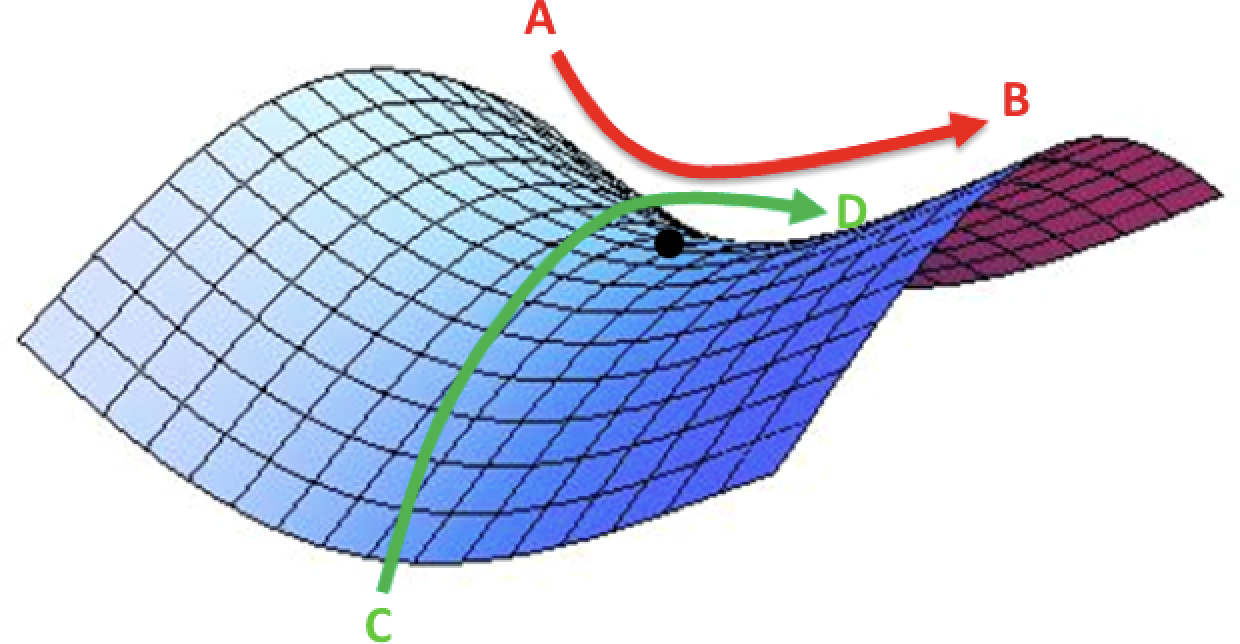
\includegraphics[width=0.6\textwidth]{saddle_point_problem.png}
\caption{Saddle point over a 3D surface \cite{Buduma_book}}
\label{fig:3.1}
\end{figure}

A better understanding of \Cref{eq:3.15.1,eq:3.15.2} can be observed in \Cref{fig:3.1}. Depending upon how one cuts the surface moving along the direction A to B or from C to D (orthogonal direction to A to B), the critical point looks like a local minima or a local maxima, but in reality it is neither. It is a saddle point. \par 

\Cref{eq:3.10} for the coupled multi-physics problem of magneto-elastic membrane in free space is a special case of the (generalized) saddle point system. Here, the conditions C1-C4 are satisfied, but not C5 which arises in the discretization of equations describing slightly compressible solids \cite{Benzi2005}.

\subsection{Numerical solution of saddle point systems}
Iterative method using preconditioners: Schur complement method. Algorithm. Use of preconditioners (AMG theory?). Use of linear operator data structure from deal.ii. \par 

Explain the LSAE for our coupled problem. The properties of each block of the matrix. Choice of the block to proceed with schur complement of that block of matrix (why phi phi block?). Precomputations performed to transform the corresponding block from neg def to pos def (for solution by use of iterative method such as CG). \par 

Direct solution method: Monolithic approach using UMFPACK. Assembly in serial block solution and rhs vectors. 

To solve the linear system of equations \Cref{eq:3.10}, one of the following approach can be taken:
\begin{itemize}
\item Direct solver solving the complete system monolithically.
\item Global iterative solver with a global preconditioner constructed for the tangent matrix $\mathbf{K}$.
\item Sequentially solve for each unknown field $\phi$ and $\mathbf{u}$ exploiting the tangent matrix's block structure.
\end{itemize}
Below we explain the direct solver and the iterative solution method exploiting the block structure that were implemented. Before we discuss the details of the solution methods, it is important to highlight the properties of each block in the tangent matrix $\mathbf{K}$. This will also explain the motive for the choice of block to proceed with iterative solution method detailed in the further section.\par 

As observed in the finite element discretized form for the coupled problem, the block for purely magnetic scalar potential contribution $\mathbf{K}_{\phi \phi} = - \int\limits_{\mathcal{D}_0} \nabla_0 N^I \cdot \mathbf{D} \cdot \nabla_0 N^J$ results in a symmetric negative-definite matrix of size $p \times p$. The block for purely non-linear elastic contribution $\mathbf{K}_{\mathbf{u} \mathbf{u}} = \int\limits_{\mathcal{D}_0} \left[ \left[ \nabla_0^T \mathbf{N}^I \cdot \nabla_0 \mathbf{N}^J \right] : \mathbf{S} + \left[ \mathbf{F}^T \cdot \nabla_0 \mathbf{N}^I \right] : \mathfrak{C} : \left[ \mathbf{F}^T \cdot \nabla_0 \mathbf{N}^J \right] \right]$ represents a symmetric positive-definite matrix of size $q \times q$. For the considered axisymmetric problem, we know that for any given total number of support points $n_d$, $p < q$ given that we solve for a single scalar-valued magnetic potential $\phi$ and a vector-valued displacement $(u_r, u_z)^T$. Thus, the size of block $\mathbf{K}_{\phi \phi}$ is always less than the block $\mathbf{K}_{\mathbf{u} \mathbf{u}}$ (unless we solve for a 1D problem). The blocks resulting from the coupling between the two fields, namely $\mathbf{K}_{\phi \mathbf{u}}$ and $\mathbf{K}_{\mathbf{u} \phi}$ are symmetric negative-definite matrices with sizes $p \times q$ and $q \times p$, respectively and are transposes of each other. Thus, one can assemble one block and store the other as the transpose of the assembled block to save computations. Due to the sparsity arising in each individual block, the structure of the tangent matrix $\mathbf{K}$ is an unsymmetric sparse banded block matrix.\par 

\subsubsection{Direct solver}
This category of solvers is also known as `\textit{coupled}' or `all at once' methods. Coupled solvers deal with the system such as \Cref{eq:3.10} as a whole, computing both the fields $\phi$ and $\mathbf{u}$ simultaneously and without making any explicit use of reduced systems. In most cases, due to the ease of implementation, the direct solver is employed. One doesn't have to care about the properties of the tangent matrix $\mathbf{K}$ and also about the properties of individual blocks. \par 

We use a sparse direct solver called UMFPACK \cite{davis2004algorithm}, which is part of the SuiteSparse library \cite{davis2015suitesparse}. Interface to this solver is provided in the \texttt{deal.II} \cite{Alzetta2018} library in the form of the class \textbf{SparseDirectUMFPACK}. UMFPACK is a set of routines for solving unsymmetric sparse linear systems of the form $\mathbf{A} \cdot \mathbf{x} = \mathbf{b}$. It employs the unsymmetric multifrontal method and direct sparse LU factorization. It is heavily used as a built-in routine in MATLAB\textsuperscript{\tiny\sffamily\textregistered} and appears as lu and $\mathbf{x} = \mathbf{A} \setminus \mathbf{b}$ (back slash operator). It is important to note that this solver is a serial solver and therefore one cannot employ parallel (MPI) data structures for the vectors and reap the benefits of distributed memory parallelism for a large system of equations. Thus, solution time for a large system using such a serial direct solver would be high compared to a parallelized iterative solver in most cases. But for our problem of interest, in axisymmetric formulation it was observed that the computation time for the total solution was comparable to that of a parallelized iterative solver mentioned in the next section.

\subsubsection{Segregated iterative solver using Schur complement reduction}
The other category of solvers is the so called segregated solver which computes both the unknown fields $\phi$ and $\mathbf{u}$ separately. This approach involves the solution of two linear systems of size smaller than $p+q$ which are termed as \textit{reduced systems}. One reduced system is formed for the field $\phi$ and the other reduced system for the field $\mathbf{u}$. Depending upon the number of unknown fields, for example, in cases of a Lagrange multiplier, a separate reduced system for that unknown field is also formed and solved. Here, we shall look at one of the representatives of such a segregated approach known as the Schur complement reduction which we implemented for the solution of the fully-coupled magneto-elastic problem of our interest. \par 

The Schur complement reduction is based on the block LU factorization of the sparse block tangent matrix $\mathbf{K}$. Consider the saddle point system of our interest  from \Cref{eq:3.10}:
\begin{equation}
\mathbf{K}_{\phi \phi} \cdot \Delta \mathbf{d}_{\phi} + \mathbf{K}_{\phi \mathbf{u}} \cdot \Delta \mathbf{d}_{\mathbf{u}} = -\mathbf{R}_{\phi}, \ \ \mathbf{K}_{\mathbf{u} \phi} \cdot \Delta \mathbf{d}_{\phi} + \mathbf{K}_{\mathbf{u} \mathbf{u}} \cdot \Delta \mathbf{d}_{\mathbf{u}} = -\mathbf{R}_{\mathbf{u}}. 
\label{eq:3.16}
\end{equation}
If the block $\mathbf{K}_{\phi \phi}$ is square and non-singular (invertible), which in our case is true, the saddle point matrix $\mathbf{K}$ admits the following block triangular factorization:
\begin{equation}
\mathbf{K} = 
\begin{bmatrix}
\mathbf{K}_{\phi \phi} & \mathbf{K}_{\phi \mathbf{u}} \\
\mathbf{K}_{\mathbf{u} \phi} & \mathbf{K}_{\mathbf{u} \mathbf{u}}
\end{bmatrix} 
= 
\begin{bmatrix}
\mathbf{I} & \mathbf{0} \\
\mathbf{K}_{\mathbf{u} \phi} \mathbf{K}_{\phi \phi}^{-1} & \mathbf{I}
\end{bmatrix}
\begin{bmatrix}
\mathbf{K}_{\phi \phi} & \mathbf{0} \\
\mathbf{0} & \mathbf{S}
\end{bmatrix}
\begin{bmatrix}
\mathbf{I} & \mathbf{K}_{\phi \phi}^{-1} \mathbf{K}_{\phi \mathbf{u}}^T \\
\mathbf{0} & \mathbf{I}
\end{bmatrix},
\label{eq:3.17}
\end{equation} 
where $\mathbf{I}$  and $\mathbf{0}$ are the unit identity matrix and null matrix of appropriate size, respectively. The matrix $\mathbf{S}$ is the Schur complement of block $\mathbf{K}_{\phi \phi}$ in $\mathbf{K}$ and is defined as:
\begin{equation}
\mathbf{S} = \mathbf{K}_{\mathbf{u} \mathbf{u}} - \mathbf{K}_{\mathbf{u} \phi} \mathbf{K}_{\phi \phi}^{-1} \mathbf{K}_{\phi \mathbf{u}} \equiv \mathbf{D} - \mathbf{C} \mathbf{A}^{-1} \mathbf{B} \ \text{from \Cref{eq:3.11}}.
\label{eq:3.18}
\end{equation}
With the magnetic potential stiffness block $\mathbf{K}_{\phi \phi}$ and the total stiffness matrix $\mathbf{K}$ being square and invertible, by the block triangular factorization in \Cref{eq:3.17} the Schur complement $\mathbf{S}$ is also invertible. Pre-multiplying both the sides of the first equation in \Cref{eq:3.16} by $\mathbf{K}_{\mathbf{u} \phi} \mathbf{K}_{\phi \phi}^{-1}$, we obtain
\begin{equation}
\mathbf{K}_{\mathbf{u} \phi} \cdot \Delta \mathbf{d}_{\phi} +  \mathbf{K}_{\mathbf{u} \phi} \mathbf{K}_{\phi \phi}^{-1} \mathbf{K}_{\phi \mathbf{u}} \cdot \Delta \mathbf{d}_{\mathbf{u}} = -\mathbf{K}_{\mathbf{u} \phi} \mathbf{K}_{\phi \phi}^{-1} \cdot \mathbf{R}_{\phi}.
\end{equation}
Using $\mathbf{K}_{\mathbf{u} \phi} \cdot \Delta \mathbf{d}_{\phi} = -\mathbf{R}_{\mathbf{u}} - \mathbf{K}_{\mathbf{u} \mathbf{u}} \cdot \Delta \mathbf{d}_{\mathbf{u}}$ from the second equation in \Cref{eq:3.16}, after rearranging we see
\begin{equation}
\left( \mathbf{K}_{\mathbf{u} \mathbf{u}} - \mathbf{K}_{\mathbf{u} \phi} \mathbf{K}_{\phi \phi}^{-1} \mathbf{K}_{\phi \mathbf{u}} \right) \cdot \Delta \mathbf{d}_{\mathbf{u}} = \mathbf{K}_{\mathbf{u} \phi} \mathbf{K}_{\phi \phi}^{-1} \cdot \mathbf{R}_{\phi} - \mathbf{R}_{\mathbf{u}} \implies \mathbf{S} \cdot \Delta \mathbf{d}_{\mathbf{u}} = \mathbf{R}_{\mathbf{u}}^',
\label{eq:3.19}
\end{equation}
with the modified right-hand side vector $\mathbf{R}_{\mathbf{u}}^' := \mathbf{K}_{\mathbf{u} \phi} \mathbf{K}_{\phi \phi}^{-1} \cdot \mathbf{R}_{\phi} - \mathbf{R}_{\mathbf{u}}$ arising from the condensation step.
In terms of the general representation as in \Cref{eq:3.11}, we arrive at
\begin{equation}
\left( \mathbf{D} - \mathbf{C} \mathbf{A}^{-1} \mathbf{B} \right) \cdot \mathbf{y} = \mathbf{g} - \mathbf{C} \mathbf{A}^{-1} \mathbf{f} \implies \mathbf{S} \cdot \mathbf{y} = \mathbf{g}^'.
\label{eq:3.20} 
\end{equation}
\Cref{eq:3.19,eq:3.20} represent a reduced system of order $q$ for the solution update in displacement field $\Delta \mathbf{d}_{\mathbf{u}}$. It is important to note that unless $-\mathbf{R}_{\phi} \equiv \mathbf{f} = \mathbf{0}$, pre-processing the condensed right-hand side vector $\mathbf{R}_{\mathbf{u}}^' \equiv \mathbf{g}^'$ requires solving another linear system of equation of the form $\mathbf{A} \cdot \mathbf{v} = \mathbf{f}$. Once the solution (or an approximation) $\Delta \mathbf{d}_{\mathbf{u}}$ of the reduced system \Cref{eq:3.19} is computed, we then post-process the solution update for the other field $\Delta \mathbf{d}_{\phi}$ using the solution from the first update $\Delta \mathbf{d}_{\mathbf{u}}$ as
\begin{equation}
\mathbf{K}_{\phi \phi} \cdot \Delta \mathbf{d}_{\phi} = -\mathbf{R}_{\phi} - \mathbf{K}_{\phi \mathbf{u}} \cdot \Delta \mathbf{d}_{\mathbf{u}}.
\label{eq:3.21}
\end{equation}
\Cref{eq:3.21} represents the other reduced system of size $p$ that needs to be solved for the magnetic potential solution update. \Cref{alg:3.1} highlights the algorithmic steps needed to solve any saddle point system using the segregated iterative solver. The algorithm is explained for the fully-coupled magneto-elastic problem of our interest, solving for the displacement field first and then for the magnetic potential, but can be applied for any general saddle point system such as \Cref{eq:3.11}.

\begin{algorithm}[h]
\begin{enumerate}
\item Define the inverse $\mathbf{K}_{\phi \phi}^{-1}$ using a solver with preconditioner.
\item Define the Schur complement $\mathbf{S} = \mathbf{K}_{\mathbf{u} \mathbf{u}} - \mathbf{K}_{\mathbf{u} \phi} \mathbf{K}_{\phi \phi}^{-1} \mathbf{K}_{\phi \mathbf{u}}$.
\item Define the inverse of the Schur complement $\mathbf{S}^{-1}$ using another solver with a preconditioner to compute the approximate inverse operation of $\mathbf{S}$. 
\item Perform the pre-processing step to condense the right-hand side vector $\mathbf{R}_{\mathbf{u}}^' := \mathbf{K}_{\mathbf{u} \phi} \mathbf{K}_{\phi \phi}^{-1} \cdot \mathbf{R}_{\phi} - \mathbf{R}_{\mathbf{u}}$.
\item Solve for the solution update $\Delta \mathbf{d}_{\mathbf{u}}$: $\Delta \mathbf{d}_{\mathbf{u}} = \mathbf{S}^{-1} \cdot \mathbf{R}_{\mathbf{u}}^'$.
\item Post-process the solution for the other field: $\Delta \mathbf{d}_{\phi} = \mathbf{K}_{\phi \phi}^{-1} \left( -\mathbf{R}_{\phi} - \mathbf{K}_{\phi \mathbf{u}} \cdot \Delta \mathbf{d}_{\mathbf{u}} \right)$. 
\end{enumerate}
\caption{Schur complement reduction}
\label{alg:3.1}
\end{algorithm}

\begin{large}
\noindent \textbf{Choice of the block to compute the Schur complement of $\mathbf{K}$:}\\
\end{large}
\indent The choice of the block $\mathbf{K}_{\phi \phi}$  of size $p \times p$ to proceed with the Schur complement of $\mathbf{K}$ is due to the small size of the block compared to the other diagonal block $\mathbf{K}_{\mathbf{u} \mathbf{u}}$ of size $q \times q$, with $p < q$ as mentioned in the previous section. The motive behind the choice of the block of small size is the need to compute the inverse of the chosen block in computing the Schur complement $\mathbf{S}$ as observed in \Cref{eq:3.18}. Computational cost of computing the inverse of a matrix of size $q \times q$ exceeds that of the cost for a matrix of size $p \times p$. One also needs to take into account the lower bandwidth of the scalar magnetic potential stiffness matrix block compared to that of the displacement stiffness matrix block \cite{Pelteret2016}. \newline \par 

Typically this inversion of the chosen block matrix is performed by using a robust Krylov subspace iterative solver such as the Conjugate Gradient method with some form of preconditioning. The CG method works on only symmetric positive-definite matrices \cite{EdwinK.P.Chong2013}. Whereas the block $\mathbf{K}_{\phi \phi}$ and $\mathbf{K}_{\phi \mathbf{u}}$ of the first equation in \Cref{eq:3.16} are symmetric negative-definite matrices. In order to compute the inverse $\mathbf{K}_{\phi \phi}^{-1}$ using the CG iterative solver we need to transform the matrix $\mathbf{K}_{\phi \phi}$ to a positive-definite matrix. We do this by multiplying the first equation in \Cref{eq:3.16} by a factor of -1. This leads to a system of equations as
\begin{equation}
-\mathbf{K}_{\phi \phi} \cdot \Delta \mathbf{d}_{\phi} - \mathbf{K}_{\phi \mathbf{u}} \cdot \Delta \mathbf{d}_{\mathbf{u}} = \mathbf{R}_{\phi},
\end{equation}
with symmetric positive-definite matrix blocks. The matrix block $\mathbf{K}_{\phi \phi}$ is preconditioned to reduce the condition number and thus have a good convergence rate within the iterative solver computing an approximation to the inverse $\mathbf{K}_{\phi \phi}^{-1}$. We have employed the Trilinos \cite{heroux2005overview} linear algebra suite for the parallel and efficient data structures of vectors, matrices, preconditioners and solvers. Jacobi, SSOR and the Algebraic Multigrid (AMG) \cite{gee2006ml} preconditioners were used from the Trilinos suite. Depending on a user input parameter one of the three would be used. To compute the inverse $\mathbf{K}_{\phi \phi}^{-1}$ a reduced-iteration CG solver was employed. The linear transformations such as the scaling of matrix with a factor of -1, forming the inverse operator $\mathbf{K}_{\phi \phi}^{-1}$ and the Schur complement $\mathbf{S}$ was carried out using the class \textbf{LinearOperator} from the \texttt{deal.II} library. Lazy evaluation of linear transformations and expressions using vectors and matrices is performed by this class. The lazy evaluation of an expression helps in avoiding any intermediate storage of temporary objects. The class stores the sequence of operations that need to be performed on the vector/matrix object and executes them only when the value of the object is required. The class \textbf{LinearOperator} provides several member functions that aid the user implementing a Schur complement reduction solver. The member function \textbf{linear\_operator()} was used on each block of the tangent matrix $\mathbf{K}$ to transform the underlying Trilinos sparse matrix to a \textbf{LinearOperator} data structure. The function \textbf{inverse\_operator()}, which takes the matrix of which inverse is to be computed, the iterative linear solver and the preconditioner for the matrix as arguments, was employed to form the inverse operator $\mathbf{K}_{\phi \phi}^{-1}$. The Schur complement was defined using the member function \textbf{schur\_complement()} which takes the four matrix blocks as arguments required to define the Schur complement $\mathbf{S} := \mathbf{D} - \mathbf{C} \mathbf{A}^{-1} \mathbf{B}$. \par 

Another reduced-iteration CG solver was used with one of the three precondtioner to define the inverse operator for the Schur complement $\mathbf{S}^{-1}$. To pre-process the condensed right-hand side vector as mentioned in \Cref{alg:3.1}, the member function \textbf{condense\_schur_rhs()} of the class \textbf{LinearOperator} was employed. To post-process the solution update for the second field the member function \textbf{postprocess\_schur_solution()} was employed. Thus, in total two different iterative solvers with respective preconditioners were implemented within the Schur complement reduction method. An inner solver to compute $\mathbf{K}_{\phi \phi}^{-1}$ and an outer solver to compute $\mathbf{S}^{-1}$.

\section{Test case and Results}
\subsection{Unit test problem}

\subsection{Torus problem}
With mechanical load applied first, followed by magnetic load. Results. Conclusion. \par 

With magnetic load applied first, followed by mechanical load (to observe mechanically induced instabilities in the membrane). Results and conclusions.


\newpage
\printbibliography
\end{document}
